
\chapter{Cross-reference}

%\begin{todo} %done
%    Move k-majority from week 5 to week 7, as it becomes important in representative democracies but is nonsense when talking about just majority rule.  Avoid discussing the two-tier problem until week 7.
%\end{todo}




\begin{figure}[ht]
    \centering
    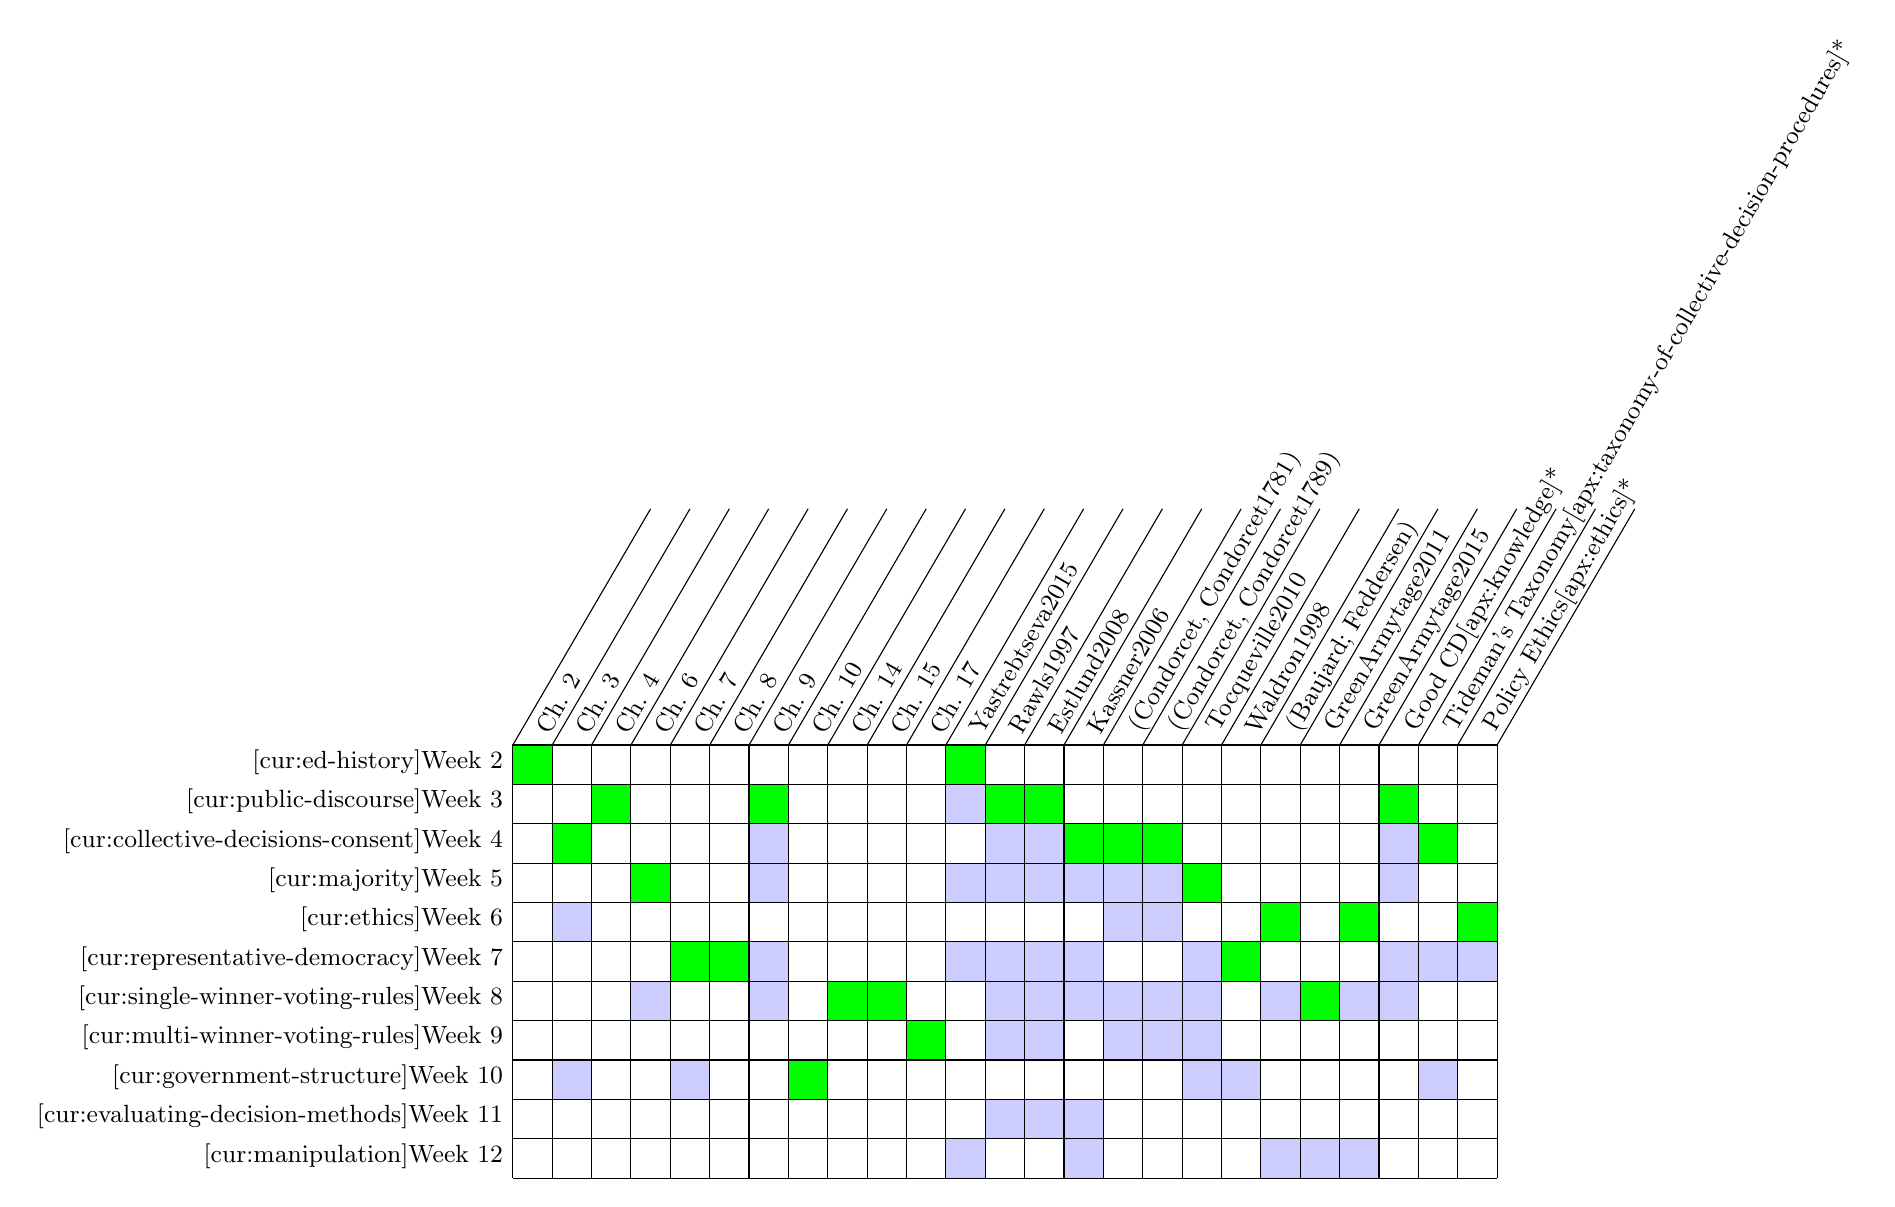
\begin{tikzpicture}[
        %sibling distance=10em,
        font=\small,
        ]
    \foreach \x[count=\xi from 0] in {
        2, % Ch. 2
        4,
        3,
        5,
        7,
        7,
        3,
        10,
        8,
        8,
        9,
        2,
        3,
        3,
        4,
        4,
        4,
        5,
        7,
        6, % Baujard and Feddersen
        8, % Condorcet-Hare
        6, % Green-Armytage,
        3, % Good CD/knowledge
        4, % Taxonomy
        6 % Ethics
    }
    {
        \draw [fill=green] (\xi/2,1-\x/2) rectangle ++(0.5,-0.5);
    }
    \foreach \x / \y in {
        1/6, 1/10,
        3/8,
        4/10,
        6/4, 6/5, 6/7, 6/8,
        11/3, 11/5, 11/7, 11/12,
        12/4, 12/5, 12/7, 12/11, 12/8, 12/9,
        13/4, 13/5, 13/7, 13/11, 13/8, 13/9,
        14/5, 14/7, 14/11, 14/8, 14/12,
        15/5, 15/6, 15/8, 15/9,
        16/5, 16/6, 16/8, 16/9,
        17/7, 17/8, 17/9, 17/10,
        18/10,
        19/8, 19/12,
        20/12,
        21/8, 21/12,
        22/4, 22/5, 22/7, 22/8, % Good CD
        23/7, 23/10,
        24/7
    }
    {
        \draw [fill=blue!20] (\x/2,1-\y/2) rectangle ++(0.5,-0.5);
    }
    \foreach \x[count=\xi] in {
        Ch. 2,
        Ch. 3,
        Ch. 4,
        Ch. 6,
        Ch. 7,
        Ch. 8,
        Ch. 9,
        Ch. 10,
        Ch. 14,
        Ch. 15,
        Ch. 17,
        \autocite{Yastrebtseva2015},
        \autocite{Rawls1997},
        \autocite{Estlund2008},
        \autocite{Kassner2006},
        {(Condorcet, \citeyear{Condorcet1781})},
        {(Condorcet, \citeyear{Condorcet1789})},
        \autocite{Tocqueville2010},
        \autocite{Waldron1998},
        {(Baujard; Feddersen)},
        \autocite{GreenArmytage2011},
        \autocite{GreenArmytage2015},
        Good CD\hyperref[apx:knowledge]{*},
        Tideman's Taxonomy\hyperref[apx:taxonomy-of-collective-decision-procedures]{*},
        Policy Ethics\hyperref[apx:ethics]{*},
        {}
    }
    {
        \node at (0.5*\xi-0.35,0) [anchor=south west] {\rotatebox{60}{\x}};
        \draw (0.5*\xi-0.5,0) -- ++(1.75,3);
        \draw (0.5*\xi-0.5,0) -- ++(0,-12/2+0.5);
    }

    \draw (0,0) -- (12.5,0);
    \foreach \x[count=\xi] in {
        \hyperref[cur:ed-history]{Week 2},
        \hyperref[cur:public-discourse]{Week 3},
        \hyperref[cur:collective-decisions-consent]{Week 4},
        \hyperref[cur:majority]{Week 5},
        \hyperref[cur:ethics]{Week 6},
        \hyperref[cur:representative-democracy]{Week 7},
        \hyperref[cur:single-winner-voting-rules]{Week 8},
        \hyperref[cur:multi-winner-voting-rules]{Week 9},
        \hyperref[cur:government-structure]{Week 10},
        \hyperref[cur:evaluating-decision-methods]{Week 11},
        \hyperref[cur:manipulation]{Week 12}
    }
    {
        \node at (0,-0.5*\xi) [anchor=south east] {\x};
        \draw (0,-0.5*\xi) -- (12.5,-0.5*\xi);
    }

    \end{tikzpicture}
    \caption{\label{fig:resources}Resources and concepts introduced and later discussed.}
\end{figure}

\section{The Handbook of Social Choice and Voting}

This course uses the Handbook of Social Choice and Voting \autocite{Heckelman2015} as its primary text.  Readings are assigned as follows:

\begin{itemize}
    \item Chapter 2:  The strange history of social choice (\hyperref[cur:ed-history]{Week 2})

    \item Chapter 3:  Unanimous consent and constitutional economics (\hyperref[cur:collective-decisions-consent]{Week 4})
    \begin{itemize}
        \item \hyperref[cur:ethics]{Ethics and Welfare}:  Consent to rules based on Pareto and Scitovsky's Double
    \end{itemize}

    \item Chapter 4:  Rational choice and the calculus of voting (\hyperref[cur:public-discourse]{Week 3})

    \item Chapter 6:  Majority rule and tournament solutions (\hyperref[cur:majority]{Week 5})

    \item Chapter 7:  Supermajority Rules (\hyperref[cur:representative-democracy]{Week 7})

    \item Chapter 8:  Measuring a-priori voting power (\hyperref[cur:representative-democracy]{Week 7})

    \item Chapter 9:  Condorcet Jury Theorem (\hyperref[cur:public-discourse]{Week 3})
    %163-180
    \item Chapter 10:  Spatial modeling (\hyperref[cur:public-government-structure]{Week 10})

    \item Chapter 14:  Arrow's theorem (\hyperref[cur:single-winner-voting-rules]{Week 8})

    \item Chapter 15:  Properties and paradoxes of common voting rules (\hyperref[cur:single-winner-voting-rules]{Week 8})

    \item Chapter 17:  Multiple-winner rules (\hyperref[cur:multi-winner-voting-rules]{Week 9})

\end{itemize}

I intentionally avoid anything having to do with modeling and computation.  This is a no-math course.

\section{Philosophy Resources}

A list of the assignments pertaining to each week, assigned before class and as follow-up to in-class discussions.

\begin{itemize}
    \item The Doctrine of Public Education of Condorcet in Light of the Discussion on Women's Rights and Slavery at the Beginning of the Third Republic \autocite{Yastrebtseva2015}
    \begin{itemize}
        \item Assigned:  \hyperref[cur:ed-history]{Education, Knowledge, and a History of Social Choice}
        \item Discussed:
        \begin{itemize}
            \item \hyperref[cur:public-discourse]{Public Discourse and Good Collective Decisions}:  The public discourse exchanges knowledge.

            \item \hyperref[cur:majority]{Majority Rule and Preferential Voting}:  Without knowledge and education, we don't even understand majority rule.

            \item \hyperref[cur:representative-democracy]{Representative Democracy}:  Individuals don't have knowledge of everything, even through the public discourse.  Instead, they rely on others to apply specialized knowledge in governing.

            \item \hyperref[cur:manipulation]{Electoral Manipulation}:  Without education, people can't examine whether their elections are democratic; the manipulate of elections, including the selection of types of elections based on partisan advantage rather than democratic merits, embodies tyranny feeding on ignorance.

            \item Anything having to do with public reason also has to do with knowledge.
        \end{itemize}
    \end{itemize}

    \item The Idea of Public Reason Revisited \autocite{Rawls1997}
    \begin{itemize}
        \item Assigned:  \hyperref[cur:public-discourse]{Public Discourse and Good Collective Decisions}
        \item Discussed:
        \begin{itemize}
            \item \hyperref[cur:collective-decisions-consent]{Collective Decisions and Consent}:  Agreement on outcome by achieved consensus is only possible by exchanging knowledge through discourse; achieved pseudo-consensus incorporates the economic decision among some individuals to simply bail out on the argument and accept a result they don't agree with because they can't win the argument.

            \item \hyperref[cur:majority]{Majority Rule and Preferential Voting}:  Majority rule creates the intersection of the public discourse when consensus—unanimous consent—isn't achievable.

            \item \hyperref[cur:representative-democracy]{Representative Democracy}:  Going along with individuals not having all knowledge, campaigns are public discourse to decide who has the correct knowledge to make decisions on our behalf.
            % TODO:  fill this out
            \item \hyperref[cur:evaluating-decision-methods]{Evaluating Decision Methods}: tba

            \item \hyperref[cur:single-winner-voting-rules]{Single-Winner Voting Rules and Elections}:  Condorcet rules in particular bring together the knowledge of all the people to find a mutually-agreeable collective decision between many alternatives, so long as the alternatives include one close to the median voter (i.e. who is running as a candidate matters).  Condorcet systems as such encourage candidates in such an ideological position to run, as there is maximum chance of victory.

            \item \hyperref[cur:multi-winner-voting-rules]{Multi-Winner Voting Rules and Elections}:  Proportional rules such as STV separate out groups of similarly-minded voters, such that multi-member districts elevate more-individualized voices to the high-visibility position of elected officials.  Legislators elected as such debate with one another and speak to the greater population from different viewpoints, enhancing the diversity of ideals surfacing in the public discourse by raising more minority views.
        \end{itemize}
    \end{itemize}

    \item Introduction: Epistemic Approaches to Democracy \autocite{Estlund2008}
    \begin{itemize}
        \item Assigned:  \hyperref[cur:public-discourse]{Public Discourse and Good Collective Decisions}
        \item Discussed:
        \begin{itemize}
            \item Same as \autocite{Rawls1997}
        \end{itemize}
    \end{itemize}

    \item Debate: Is Everything Really Up for Grabs? The Relationship between Democratic Values and a Democratic Process \autocite{Kassner2006}
    \begin{itemize}
        \item Assigned:  \hyperref[cur:collective-decisions-consent]{Collective Decisions and Consent}
        \item Discussed:
        \begin{itemize}
            \item \hyperref[cur:majority]{Majority Rule and Preferential Voting}:  Process vs. Principles as we look at the question of what is a majority.
            \item \textit{Every discussion where we show flaws in the electoral process and raise questions about e.g. median voter theorem is going to reference this}

            \item \hyperref[cur:representative-democracy]{Representative Democracy}:  Representative democracy is important, and still raises important questions, notably around 2-tier representation and k-majority votes in the Senate (both from the question of whether k-majority's ability to find better consensus is more democratic in general and whether it appropriately addresses two-tier representation issues).
            % TODO:  fill this out
            \item \hyperref[cur:evaluating-decision-methods]{Evaluating Decision Methods}: tba

            \item \hyperref[cur:single-winner-voting-rules]{Single-Winner Voting Rules and Elections}:  Failures in IRV and party primary election cycles represent mass disenfranchisement.  Condorcet and Smith-efficient methods appears to cover for this, if and only if some Smith candidates survive the primary process.  Borda's ability to elect a non-majority winner if the majority winner has sufficiently little support and is heavily-disliked may represent a more democratic process than even Condorcet, except Borda tends to heavily distort, which may make the process violate democratic principles in practice.

            \item \hyperref[cur:multi-winner-voting-rules]{Multi-Winner Voting Rules and Elections}:  Proportional rules such as STV enhance representation for more vioces.  These rules also reduce the disenfranchisement in a majoritarian process, which both only elevates the median voice and can suppress voters by mixing them as a minority into different voting districts.

            \item \hyperref[cur:manipulation]{Electoral Manipulation}:  Obvious concerns about an easily-manipulated election process's ability to uphold democratic principles.
        \end{itemize}
    \end{itemize}

    \item Condorcet Reflections on Negro Slavery \autocite{Condorcet1781}
    \begin{itemize}
        \item Assigned:  \hyperref[cur:collective-decisions-consent]{Collective Decisions and Consent}
        \item Discussed:  anywhere slavery comes up
        \begin{itemize}
            \item \hyperref[cur:majority]{Majority Rule and Preferential Voting}:  Slaves can't vote.

            \item \hyperref[cur:ethics]{Ethics and Welfare}:  Pareto improvements versus the ongoing injustice of slavery; Condorcet concludes slaveholders are not deprived of property when slaves are emancipated because they don't rightly own any person.

            \item \hyperref[cur:representative-democracy]{Representative Democracy}:  In America, States were afforded a census count of $\nicefrac{3}{5}$ per each enslaved person, increasing their apportioned representation in the Congress; yet these people were imagined as property and thus had no opportunity to communicate with their so-called representatives or to cast their own vote.

            \item \hyperref[cur:single-winner-voting-rules]{Single-Winner Voting Rules and Elections}:  Slavery gets a mention for excluding people regardless of the equality of vote provided by any voting rule.  Ties to further suppression of black voters.

            \item \hyperref[cur:multi-winner-voting-rules]{Multi-Winner Voting Rules and Elections}:  Also gets a mention in passing when bridging to further suppression of black voters.

        \end{itemize}
    \end{itemize}

    \item Condorcet On the Admission of Women to the Rights of Citizenship \autocite{Condorcet1789}
    \begin{itemize}
        \item Assigned:  \hyperref[cur:collective-decisions-consent]{Collective Decisions and Consent}
        \item Discussed:  same places as slavery, for similar reasons
        \begin{itemize}
            \item \hyperref[cur:majority]{Majority Rule and Preferential Voting}:  Can't take advantage of the epistemic advantages of democracy if you exclude people.
        \end{itemize}
    \end{itemize}

    \item Democracy in America: historical-critical edition of De la Démocratie en Amérique \autocite{Tocqueville2010}
    \begin{itemize}
        \item Assigned:  \hyperref[cur:majority]{Majority Rule and Preferential Voting}
        \item Discussed:
        \begin{itemize}
            \item \hyperref[cur:representative-democracy]{Representative Democracy}:  Two-tier problem and k-majority in reference to tyranny of the majority.

            \item \hyperref[cur:single-winner-voting-rules]{Single-Winner Voting Rules and Elections}:  Condorcet rules provide a direct answer to Tocqueville's tyranny of the majority.

            \item \hyperref[cur:multi-winner-voting-rules]{Multi-Winner Voting Rules and Elections}:  Proportional rules may have impact on the tyranny of the majority in the sense of the public discourse, but may still produce solid majority coalitions in legislatures.

            \item \hyperref[cur:government-structure]{Government Structure}:  Complex considerations about how the government's structure—the three-branch checks-and-balances system, unicameral vs. bicameral legislatures, and so forth—may affect the tyranny of the majority.
        \end{itemize}
    \end{itemize}

    \item Waldron on judicial review \autocite{Waldron1998}
    \begin{itemize}
        \item Assigned: \hyperref[cur:representative-democracy]{Representative Democracy}
        \item Discussed:
        \begin{itemize}
            \item \hyperref[cur:government-structure]{Government Structure}:  Checks and balances, with the courts reviewing the legislature and the executive, the executive appointing the judges of the courts with the consent of the legislature, the legislature able to impeach and remove individual judges of the courts, and the voters able to frequently decide whether to replace the executive and legislators.
        \end{itemize}
    \end{itemize}

    \item Habermas:  Three Normative Models of Democracy \autocite{Habermas1994}
    \begin{itemize}
        \item Assigned:
    \end{itemize}

    \item Baujard's piece on score voting \autocite{Baujard2014}
    \begin{itemize}
        \item Assigned:  \hyperref[cur:ethics]{Ethics and Welfare}
        \item Discussed:
        \begin{itemize}
            \item \hyperref[cur:single-winner-voting-rules]{Single-Winner Voting Rules and Elections}:  Comes up when talking about welfare systems like Borda or Score.
        \end{itemize}
    \end{itemize}

    \item Feddersen's piece on score voting \autocite{Feddersen2009}
    \begin{itemize}
        \item Same as Baujard's
    \end{itemize}

\end{itemize}